\documentclass[a4paper,12pt,oneside]{book}

%-------------------------------Start of the Preable------------------------------------------------
\usepackage[english]{babel}
\usepackage{blindtext}
%packagr for hyperlinks
\usepackage{hyperref}
\hypersetup{
    colorlinks=true,
    linkcolor=blue,
    filecolor=magenta,      
    urlcolor=cyan,
}

\urlstyle{same}
%use of package fancy header
\usepackage{fancyhdr}
\setlength\headheight{26pt}
\fancyhf{}
%\rhead{
\includegraphics[width=1cm]{logo}}
\lhead{\rightmark}
\rhead{
\includegraphics[width=1cm]{logo}}
\fancyfoot[RE, RO]{\thepage}
\fancyfoot[CE, CO]{\href{http://www.e-yantra.org}{www.e-yantra.org}}

\pagestyle{fancy}

%use of package for section title formatting
\usepackage{titlesec}
\titleformat{\chapter}
  {\Large\bfseries} % format
  {}                % label
  {0pt}             % sep
  {\huge}           % before-code
 
%use of package tcolorbox for colorful textbox
\usepackage[most]{tcolorbox}
\tcbset{colback=cyan!5!white,colframe=cyan!75!black,halign title = flush center}

\newtcolorbox{mybox}[1]{colback=cyan!5!white,
colframe=cyan!75!black,fonttitle=\bfseries,
title=\textbf{\Large{#1}}}

%use of package marginnote for notes in margin
\usepackage{marginnote}

%use of packgage watermark for pages
%\usepackage{draftwatermark}
%\SetWatermarkText{
\includegraphics{logo}}
\usepackage[scale=2,opacity=0.1,angle=0]{background}
\backgroundsetup{
contents={
\includegraphics{logo}}
}

%use of newcommand for keywords color
\usepackage{xcolor}
\newcommand{\keyword}[1]{\textcolor{red}{\textbf{#1}}}

%package for inserting pictures
\usepackage{graphicx}

%package for highlighting
\usepackage{color,soul}

%new command for table
\newcommand{\head}[1]{\textnormal{\textbf{#1}}}


%----------------------End of the Preamble---------------------------------------


\begin{document}

%---------------------Title Page------------------------------------------------
\begin{titlepage}
\raggedright
{\Large eYSIP2016\\[1cm]}
{\Huge\scshape Object Tracking Camera \\[.1in]}
\vfill
\begin{flushright}
{\large Abhishek Rathore \\}
{\large Gopineedi Harsha Vardhan \\}
{\large \textbf{Mentors:} \\}
{\large Akshat Jain \\}
{\large Pushkar Raj \\}
{\large Rama kumar \\}
{\large Duration of Internship: $ 21/05/2016-10/07/2016 $ \\}
\end{flushright}

{\itshape 2016, e-Yantra Publication}
\end{titlepage}
%-------------------------------------------------------------------------------

\chapter[Project Tag]{Object Tracking Camera}
\section*{Abstract}
Object tracking is the process of locating a moving object over time using a camera. It has a variety of uses, some of which are: human-computer interaction, security and surveillance, video communication and compression, augmented reality, traffic control, medical imaging and video editing. Object tracking can be a time consuming process due to the amount of data that is contained in each frame.
 \par The objective of Object tracking is to associate target object in consecutive video frames. The association can be especially difficult when the object is moving fast relative to the frame rate. Another situation that increases the complexity of the problem is when the tracked object changes orientation over time.
 \par This system will track an object given through a Region-Of-interest using Real-Time Image Processing.The project starts with learning basic Image processing techniques and Object tracking techniques and in later stages,Advanced tracking techniques are experimented and implemented. 

\subsection*{Completion status}
The task of detecting and tracking a object using a camera is done \textbf{sucessfully}.The tasks of integrating the camera on the autonomous drone and GUI appplication for the system is yet to be done.We completed all of the tasks given to us and uploaded the tutorials on \href{https://github.com/eYSIP-2016/Object-Tracking-Camera}{GitHub}
The Tutorials done are as follows:
\begin{itemize}
 \item \textbf{Colored Object Tracking using HSV:}Tracks a colored ball by taking it HSV color range as its input and tracks the colored object by finding the largest area contour in the frame which will be our object.
 \item \textbf{Object Tracking(Based on ROI):}Tracks any object which is given in the ROI(taken through mouse) by CAM SHift Algorithm using Histograms and back-projections of the object.
 \item \textbf{Tutorial on Gimbal making:}Explains on how to choose Gimbal and its parts for the drone ,how to select best low-weight parts and designing the gimbal.
 \item \textbf{Re-recognizing the Object:}Re-recognizes the object if it gets lost out of the frame comparing the back-projection of the object with the whole frame and searches for the object when it gets lost
 \item \textbf{Setting Up Raspberry-Pi:}Installing necessary python packages required for tracking and camera packages.Interfacing the servos with the GPIO pins of R-Pi.
 \item \textbf{Object Tracking Camera interfaced on a Raspberry-Pi:}Cam Shift algorithm and Re-recognizing algorithms are implemented on the R-pi which has a interfaced Object tracking camera on it.Thi system tracks any object given through a ROI.
 \end{itemize}

\section{Hardware parts}
\begin{itemize}
  \item Raspberry Pi B+
\href{https://github.com/eYSIP-2016/Autonomous-Drone/blob/master/datasheets/raspberry%20pi%20B%2B.pdf}{Datasheet}
  \item Raspberry-Pi Camera module
  \href{https://www.raspberrypi.org/wp-content/uploads/2013/07/RaspiCam-Documentation.pdf}{Datasheet}
  \item 3-D printed Camera mount frame
  \href {https://github.com/eYSIP-2016/Object-Tracking-Camera/blob/master/Tutorials/5.%20Interfacing%20the%20Camera%20and%20Gimbal%20System%20with%20the%20Raspberry-Pi/frame.jpg}{Image}
  \item Tower Pro Micro servo 9g (2 No.)
  \href {http://www.micropik.com/PDF/SG90Servo.pdf}{Datasheet}
  \item Connecting wires
  \item External Power supply
\end{itemize} 
\section{Software used}
\begin{itemize}
  \item \href{https://www.python.org/downloads}{Python 2.7.5}
  \newline \textbf{Python Packages}
  \begin{enumerate}
       \item \href{http://opencv.org/downloads.html}{Open CV 2.4.}
       \item \href{http://opencv.org/downloads.html}{numpy 1.7.1}
       \item \href{https://pypi.python.org/pypi/RPIO}{RPIO}
       \item \href{https://pypi.python.org/pypi/picamera/1.1}{Picamera}
  \end{enumerate}
  \item \href{http://mobaxterm.mobatek.net/download.html}{MobaXterm 9.0}
\end{itemize}

\section{Assembly of hardware}
\subsection{Setting up Raspberry-Pi}
		\par We will be using the Raspberry-Pi remotely from our Laptop/PC using SSH connection by MobaXterm using a LAN Cable or by a Wi-fi module that is setup on the Pi.Make sure that the Pi is connected to the Internet as we need to install necessary packages for further setup.
		\par In our case,we connected to the Pi through LAN by assigning it a static IP from the "cmdline.txt" file on the SD card.We are accessing the Internet through the Wi-fi module.
		\par It is also possible to overclock the R-Pi externally through the "config.txt" file from the SD card or internally through the "/boot/config" file.The need for overclocking is to meet the excessive processing needs of our Gimbal system.(Although it is not recommended as it may cause heating problems).
		\par In our case,we overclocked the R-Pi from 700 Mhz(default) to 900 Mhz.
		
		\subsection{Setting up Camera(Pi-Cam)}
		After fixing the Pi-cam in its connector located between the Ethernet port and HDMI port,boot up your Raspberry-Pi and open the terminal and run the following command and enable the camera(if not enabled) and reboot ur R-Pi.
		\begin{center}
			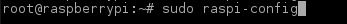
\includegraphics[scale=0.6]{cmd.png}
		\end{center}
		\begin{center}
		   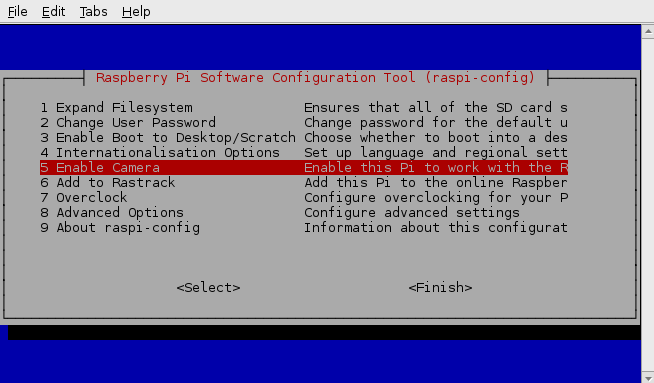
\includegraphics[scale=0.6]{enablecam.png}
		\end{center}
		\par We can check the working status of the camera by using "raspistill -o image.jpg" which takes a picture with the camera and stores it in image.jpg. 
	
		\subsection{Setting up the Pan-Tilt System}
		For making the Pan-Tilt system we will be using Two Tower Pro Servo Motors each weighing 9g (we used micro servos as they would draw a little amount of current which can be produced by the R-Pi itself)
		  \begin{center}
		   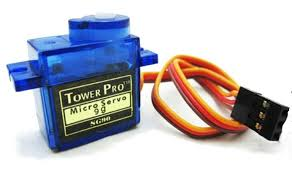
\includegraphics[scale=0.5]{servo.jpg}
		\end{center}
		\par We connected the first servo to the Pin 16(GPIO 23) and second servo to Pin 18(GPIO 24) on the board.We use this pins as signal channels when we use the servos from R-Pi.All the available GPIO ports that can be used are shown below.
		 \begin{center}
		   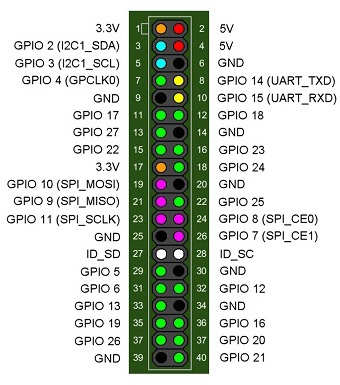
\includegraphics[scale=0.6]{gpio.jpg}
		\end{center}
		\par We calibrated each of the motor's PWM values(explained in the later section) and assembled to the frame mount which is shown below.
		  \begin{center}
		   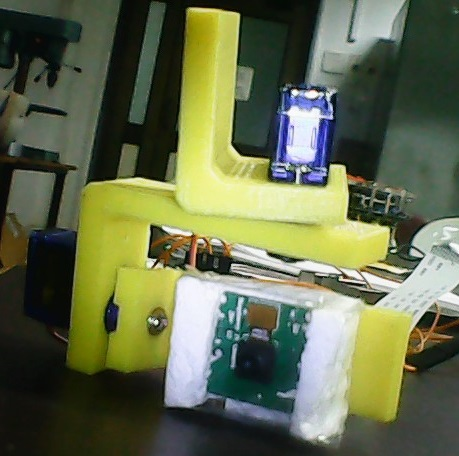
\includegraphics[scale=0.6]{frame.jpg}
		\end{center}



\section{Software and Code}
Python codes for different modules are provided below.
\begin{itemize}
    \item \href{https://github.com/eYSIP-2016/Object-Tracking-Camera/blob/master/Tutorials/1.%20Colored%20object%20tracking%20using%20HSV/Colored_object_tracking_using_HSV.py}{Color Object tracking using HSV color space}
    \item \href{https://github.com/eYSIP-2016/Object-Tracking-Camera/blob/master/Tutorials/2.%20Object%20tracking%28Based%20on%20ROI%29/Colored_Object_tracking_based_on_ROI_selection.py}{Object Tracking using a ROI}
    \item \href{https://github.com/eYSIP-2016/Object-Tracking-Camera/blob/master/Tutorials/4.%20Re-recognizing%20the%20object%20if%20it%20escapes%20and%20comes%20back%20into%20the%20frame.%20Tutorial%20on%20algorithm%20used/code.py}{Re-recognising the object if it goes out of the frame}
    \item \href{https://github.com/eYSIP-2016/Object-Tracking-Camera/blob/master/Tutorials/6.%20Object%20%20Tracking%20using%20a%20Pi-Cam%20interfaced%20on%20a%20Raspberry-Pi/code.py}{Object Tracking using a Pi-Cam interfaced on a Raspberry-Pi}
\end{itemize}
Brief explanation of various parts is done in code.

Interfacing the hardware and other modules can be found in the project page on \href{https://github.com/eYSIP-2016/Object-Tracking-Camera}{GitHub}

\section{Use and Demo}
\begin{itemize}
    \item \href{https://youtu.be/hWcxEkWLm9o}{Demo for Colored object tracking using HSV }
    \item \href{https://youtu.be/bytE1EegAfg}{Demo for Object tracking using ROI}
    \item \href {https://youtu.be/M2SsABMLuCQ}{Demo for Re-recognizing the object if it escapes from the frame}
    \item \href{https://youtu.be/8CXhzPhfl64}{Demo for Object tracking camera interfaced on a Raspberry-Pi using servo motors}
\end{itemize}

\section{Future Work}
\subsection{Hardware}
\begin{itemize}
    \item The Camera mount frame can be further developed into a Gimbal system which can be mounted on a drone
    \item The servos can be replaced with Brush-less DC motors which are much smoother.
    \item Camera with much better resolution for high end image processing might be equipped.
\end{itemize}
\subsection{Software}
\begin{itemize}
    \item More effective Object tracking algorothms can be used.
        \begin{enumerate}
            \item Key point matching can be implemented(Contiguous Match Tracker algorithm can be further improved and implemnted here)
            \item Small amount of training can be used for strong tracking of the object
            \item Multiple Tracking methods can be collaborated so that object never gets lost.
            \item Code improvements in present one
        \end{enumerate} 
    \item Servo movement can be speeded up by effective algorithms
    \item PWM controller can be implemented for balancing the gimbal effectively when mounted on a drone.
\end{itemize}
\section{Bug report and Challenges}
\subsection{Challenges faced}
 \textbf{Hardware:}
 \begin{itemize}
  \item Interfacing the servos with the GPIO pins on the Raspberry-Pi and removing their jitters.
   \item Power requirement of the servos and the camera system from the Raspberry-Pi is high.
 \end{itemize}
 \vspace{0.3cm}
 \textbf{Software:}
 \begin{itemize}
     \item Re-detection of object when it escapes from the frame
     \item Movement of camera tracking the object as both camera and object are searching for the same center.
     \item The track window for CAM shift will be shifted as the camera moves away from the current track window.
 \end{itemize}
 \subsection{Bugs}
  \begin{itemize}
   \item The algorithm cannot track high texture objects as it uses HSV color space for back projection .
   \item The camera is assumed to have the previous track window at its center which is only possible if the servos are working properly.
   \item The Camera has a low resolution which makes image processing harder and may not provide best results.
  \end{itemize}
 \section{Referred research-papers}
 \begin{itemize}
     \item \href{http://www.cv-foundation.org/openaccess/content_cvpr_workshops_2014/W18/papers/Maresca_The_Matrioska_Tracking_2014_CVPR_paper.pdf}{Matrioska Algorithm}
     \item \href{http://kahlan.eps.surrey.ac.uk/featurespace/tld/Publications/2011_tpami}{TLD-Tracker}
     \item \href{http://www.jku.at/cg/content/e60566/e155475/e155539/FRCAMShift.pdf}{CAM Shift}
     \item \href{https://e-pub.uni-weimar.de/opus4/files/1410/CAMSHift.pdf}{extended CAM Shift}
     \item \href{http://isyou.info/inpra/papers/inpra-v2n2-05.pdf}{CAMShift improvised}
     \item \href{http://www.gnebehay.com/cmt/}{CMT}
 \end{itemize}
  
\section{References}
\begin{itemize}
    \item http://www.pyimagesearch.com/2015/05/25/basic-motion-detection-and-tracking-with-python-and-opencv/
    \item http://www.theverge.com/2016/3/1/11134130/dji-phantom-4-drone-autonomous-avoidance-tracking-price-video
    \item https://oscarliang.com/build-brushless-camera-gimbal-handheld-quadcopter/
    \item https://oscarliang.com/servo-brushless-camera-gimbal-fpv-quadcopter/
    \item http://www.pyimagesearch.com/2015/09/21/opencv-track-object-movement/
    \item http://www.openelectrons.com/forums/viewtopic.php?f=4&t=6
    \item https://www.youtube.com/watch?v=PVWyZse9z4E
    \item https://www.youtube.com/watch?v=C95bngCOv9Q
    \item https://www.youtube.com/watch?v=W2qR60hrD2w
    \item https://www.youtube.com/watch?v=1GhNXHCQGsM
    \item http://blog.christianperone.com/2015/01/real-time-drone-object-tracking-using-python-and-opencv/
    \item http://ardupilot.org/copter/docs/common-camera-gimbal.html
    \item https://code.google.com/archive/p/ardupirates/wikis/StabilizedCameraMount.wiki
    \item http://www.lfd.uci.edu/~gohlke/pythonlibs/#scipy
    \item http://www.instructables.com/id/Pan-Tilt-face-tracking-with-the-raspberry-pi/step4/Connecting-the-servos/
    \item https://create.arduino.cc/projecthub/junejarohan/ball-tracking-robot-7a9865?ref=tag&ref_id=robots&offset=11
    
    
\end{itemize}



\end{document}


